%%%%%%%%%%%%%%%%%%%%%%%%%%%%%%%%%%%%%%%%%%  不使用 authblk 包制作标题  %%%%%%%%%%%%%%%%%%%%%%%%%%%%%%%%%%%%%%%%%%%%%%
%-------------------------------PPT Title-------------------------------------
\title{12 多重散射与\rm{MTO}方法}
%-----------------------------------------------------------------------------

%----------------------------Author & Date------------------------------------
%\author[\textrm{Jun\_Jiang}]{姜\;\;骏\inst{}} %[]{} (optional, use only with lots of authors)
%% - Give the names in the same order as the appear in the paper.
%% - Use the \inst{?} command only if the authors have different
%%   affiliation.
%\institute[BCC]{\inst{}%
\institute[Gain~Strong]{\inst{}%
%\vskip -20pt 北京市计算中心}
\vskip -20pt {\large 格致斯创~科技}}
\date[\today] % (optional, should be abbreviation of conference name)
{%	{\fontsize{6.2pt}{4.2pt}\selectfont{\textcolor{blue}{E-mail:~}\url{jiangjun@bcc.ac.cn}}}
\vskip 45 pt {\fontsize{8.2pt}{6.2pt}\selectfont{%清华大学\;\;物理系% 报告地点
	\vskip 5 pt \textrm{2023.05.13}}}
}

%% - Either use conference name or its abbreviation
%% - Not really information to the audience, more for people (including
%%   yourself) who are reading the slides onlin%%   yourself) who are reading the slides onlin%%   yourself) who are reading the slides onlineee
%%%%%%%%%%%%%%%%%%%%%%%%%%%%%%%%%%%%%%%%%%%%%%%%%%%%%%%%%%%%%%%%%%%%%%%%%%%%%%%%%%%%%%%%%%%%%%%%%%%%%%%%%%%%%%%%%%%%%

\subject{}
% This is only inserted into the PDF information catalog. Can be left
% out.
%\maketitle
\frame
{
%	\frametitle{\fontsize{9.5pt}{5.2pt}\selectfont{\textcolor{orange}{“高通量并发式材料计算算法与软件”年度检查}}}
\titlepage
}
%-----------------------------------------------------------------------------

%------------------------------------------------------------------------------列出全文 outline ---------------------------------------------------------------------------------
%\section*{}
%\frame[allowframebreaks]
%{
%  \frametitle{Outline}
%%  \frametitle{\textcolor{mycolor}{\secname}}
%  \tableofcontents%[current,currentsection,currentsubsection]
%}
%%在每个section之前列出全部Outline
%%类似的在每个subsection之前列出全部Outline是\AtBeginSubsection[]
%\AtBeginSection[]
%{
%  \frame<handout:0>%[allowframebreaks]
%  {
%    \frametitle{Outline}
%%全部Outline中,本部分加亮
%    \tableofcontents[current,currentsection]
%  }
%}

%-----------------------------------------------PPT main Body------------------------------------------------------------------------------------
\small
%\section{\rm{VASP~}软件中\rm{PAW~}计算的实现}
%\frame
%
%	\frametitle{\textrm{VASP}计算的特色}
%	相比于与普通的第一原理计算软件,\textrm{VASP}很好地平衡了计算效率和精度的问题,总的来说,\textrm{VASP}主要通过这几个特色保证了计算的高效能
%	\begin{itemize}
%	     \item 迭代与优化算法的多样性\\
%		     本质上电荷密度迭代 \textrm{\&\&} 体系总能量优化是相同的优化问题,采用了类似的算法\upcite{CMS6-15_1996,PRB54-11169_1996}:\\
%			\textcolor{blue}{\textrm{Pseudo-Newton、Conjugate-Gradient、Broyden~mix、damping-factor、RMM-DIIS}}
%	     \item 尽可能采用局域基(原子轨道基)函数:~\\
%		     \textcolor{blue}{\textrm{LREAL}}=\textcolor{red}{\textrm{.TRUE.}}\\
%			优化的投影函数也尽可能在实空间表示
%	     \item \textrm{PAW}原子数据集:\textcolor{blue}{优异的赝势}\upcite{PRB59-1758_1999}
%	\end{itemize}
%}
\frame
{
	\frametitle{多重散射理论}
\begin{figure}[h!]
	\vspace{-11pt}
\centering
\animategraphics[autoplay, loop, height=1.0in]{1}{Figures/Multi_scattering-}{0}{9}
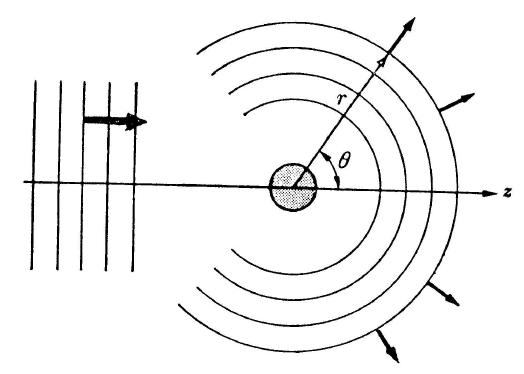
\includegraphics[height=1.29in,width=1.91in,viewport=0 0 400 275,clip]{Figures/Pseudo-scatter.jpg}
\caption{\fontsize{5.5pt}{4.2pt}\selectfont{\textrm{Schematic illustration of scattering of a plane wave by a spherical potential.}}}%(与文献\cite{EPJB33-47_2003}图1对比)
\label{Multiple_scattering}
\end{figure}
\vspace*{-0.10in}
\fontsize{7.5pt}{6.2pt}\selectfont{
	入射平面波用球\textrm{Bessel}函数展开
$$\mathrm{e}^{\mathrm{i}\vec q\cdot\vec r}=4\pi\sum_{lm}\mathrm{i}^lj_l(\vec q\cdot\vec r)Y_{lm}^{\ast}(\hat{\vec q})Y_{lm}(\hat{\vec r})=\sum_{l}(2l+1)\mathrm{i}^lj_l(qr)P_{l}(\cos\theta)$$
%$$\mathrm{e}^{\mathrm{i}\vec q\cdot\vec r}=\mathrm{e}^{\mathrm{i}qr\cos(\theta)}=\sum_{l}(2l+1)\mathrm{i}^lj_l(qr)P_{l}[\cos(\theta)]$$
}
}

\frame
{
	\frametitle{势阱与相移}
\begin{figure}[h!]
\centering
\vspace*{-0.26in}
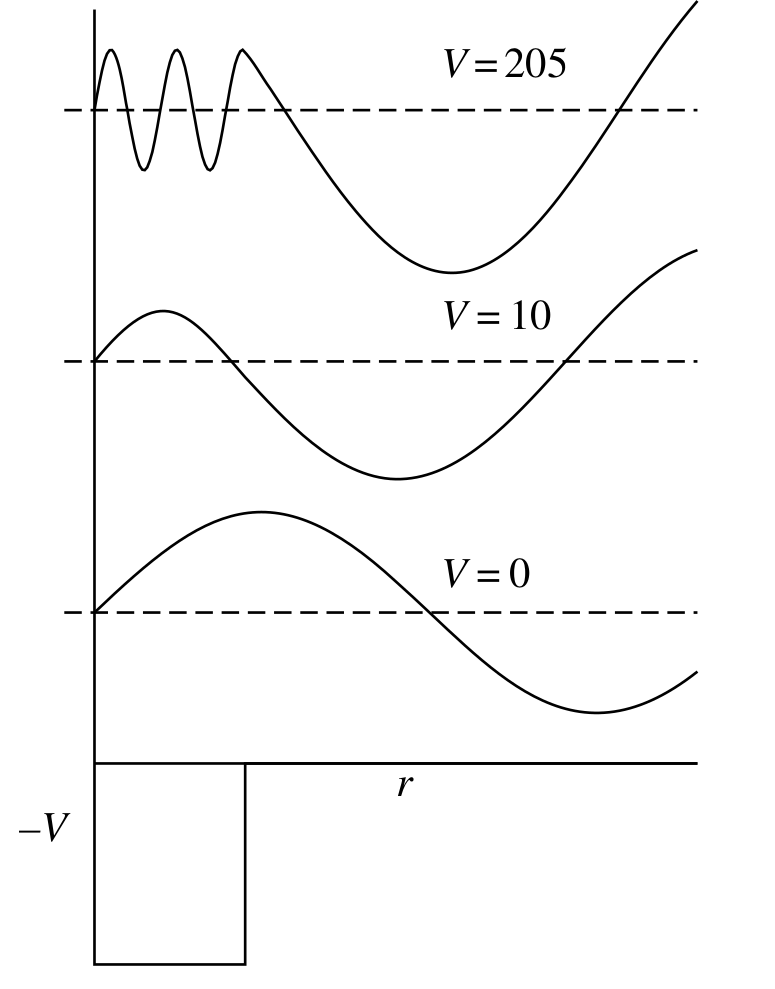
\includegraphics[height=1.85in,width=1.3in,viewport=0 0 750 1050,clip]{Figures/Radial_wave_functions_for_various_square_well_potential.png}
\caption{\fontsize{5.5pt}{4.2pt}\selectfont{\textrm{The radial wave functions for \textit{l}=0 for various square well potential depths.}}}%(与文献\cite{EPJB33-47_2003}图1对比)
\label{Pseudo-scatter}
\end{figure}
\vspace*{-0.1in}
\fontsize{7.5pt}{6.2pt}\selectfont{
平面波经散射后出射,波函数变为
$$\Psi_l^{>}(\varepsilon,r)=C_l\bigg[j_l(\kappa r)-\tan\eta_l(\varepsilon)n_l(\kappa r)\bigg]\quad\text{其中}\kappa^2=\varepsilon$$
根据散射理论,能量为$\varepsilon$的电子经单个势阱散射偏转$\theta$后,波函数的振幅可以表示为
	\begin{displaymath}
		t(\theta)=\dfrac{4\pi}{\kappa}\sum_l(2l+1)[\mathrm{exp}(2\mathrm{i}\eta_l(\varepsilon))-1]P_l(\cos\theta)
	\end{displaymath}
%$$t(\theta)=\dfrac{4\pi}{\sqrt\varepsilon}\sum_l(2l+1)\bigg[\mathrm{e}^{2\mathrm{i}\eta_l(\varepsilon)}-1\bigg]P_l(\cos\theta)$$
%$$\eta_l(\varepsilon)=p_l\pi+\delta_l(\varepsilon)$$
}
}

\section{\rm{MTO~}与\rm{LMTO~}方法}
\frame
{
\frametitle{\textrm{MTO}方法}
\textrm{MTO (Muffin-tin Orbial)}方法是\textrm{Andersen}于\textrm{1971}年提出的局域缀加基函数方案\upcite{Andersen_Book}
%\textrm{MTO}的
\vskip 5pt
\textcolor{blue}{目的:~用最小基组方法解析电子结构}
\begin{itemize}
	\item \textcolor{red}{物理图像}:~和\textrm{APW}方法类似,要求基函数在\textrm{MT}球内、外分区域表示,并且在球面上连续
	\item \textcolor{red}{数学形式}:~基函数是最小优化基组
\end{itemize}
\begin{figure}[h!]
	\vspace{-5pt}
\centering
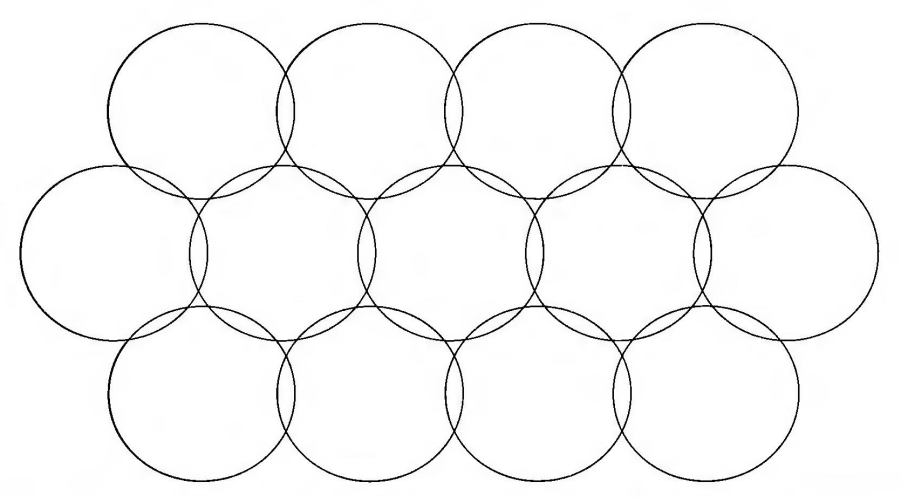
\includegraphics[height=1.20in,width=2.42in,viewport=5 0 1005 495,clip]{Figures/Atomic_sphere-appro.png}
\caption{\fontsize{6.2pt}{4.2pt}\selectfont\textrm{Atomic sphere approximation (ASA) in which the MT spheres are chosen to have the same volume as the Wigner-Seitz cell, which leads to overlapping spheres.}}
\label{Atomic_sphere-appro}
\end{figure}
}

\frame[allowframebreaks]
{
	\frametitle{\textrm{MTO-ASA}的函数形式}
		\begin{enumerate}
			\item 根据\textrm{Wigner-Seitz}理论\upcite{PR43-804_1933},将晶体划分为\textrm{Wigner-Seitz}元胞后,如果每个元胞内的势具有球形对称,则对应能量$\varepsilon$,\textrm{Schr\"odinger}方程解的形式为
				$$\psi_L(\varepsilon,\vec r)\equiv\mathrm{i}^lu_l(\varepsilon,\vec r)Y_L(\hat{\vec r})$$
				其中$u_l$是径向\textrm{Schr\"odinger}方程的解,含有相因子$\mathrm{i}^l$是因为球谐函数的\textrm{Condon-Shortley}法则\upcite{Condon-Shortley}。
%			晶体中价电子波函数的形式为
%				\begin{displaymath}
%					\Psi_{\vec k}(\vec r, \varepsilon)=\sum_LC_L(\vec k)\sum_{\vec R}\mathrm{e}^{\mathrm{i}\vec k\cdot\vec R}\theta(\vec r-\vec R)\psi_L(\varepsilon,\vec r-\vec R)
%				\end{displaymath}
%				这里$\vec R$是格矢,$\theta(\vec r)$阶梯函数,在\textrm{Wigner-Seitz}取为$1$,在\textrm{Wigner-Seitz}元胞外为$0$。

				对于给定的$\varepsilon$%和$\vec k$,调整系数$C_L$使得$\Psi_{\vec k,\varepsilon}$
				要求波函数在每个\textrm{Wigner-Seitz}元胞表面上连续到一阶。
		%	\item \textrm{MT}根据散射理论,\textrm{MT}球外基函数形如$$\psi_l(\varepsilon,\vec r)\propto j_l(q_0r)-\tan(\eta_l(\varepsilon))n_l(q_0r)$$

在原子球近似\textrm{(ASA)}下,该连续条件简化为要求径向分波$u_l(\varepsilon,r)$在球面$r=S$位置的对数导数$D_l(\varepsilon)$连续
	\begin{displaymath}
		D_l(\varepsilon)\equiv S\dfrac{u_l^{\prime}(\varepsilon,S)}{u_l(\varepsilon,S)}
	\end{displaymath}
	其中球半径取为$S=\sqrt[3]{\frac{3\Omega_0}{4\pi}}$,$\Omega_0$是\textrm{Weiger-Seitz}元胞

\item \textrm{Wigner-Seitz}元胞内取近似球形势是很粗糙的,\textrm{Slater}引入\textrm{MT}球近似,假设间隙区的势是常数$V_{\mathrm{MT}}^I$,则间隙区电子动能为
				\begin{displaymath}
					q_0^2=\varepsilon-V_{\mathrm{MT}}^I
				\end{displaymath}
				如果间隙区的势$V_{\mathrm{MT}}^I(\vec r)=0$,径向波函数满足
				\begin{displaymath}
					\bigg[-\dfrac{\mathrm{d}^2}{\mathrm{d}r^2}+\dfrac{l(l+1)}{r^2}-q_0^2\bigg]ry_l(q_0r)=0
				\end{displaymath}
				根据散射理论,散射后波函数%渐近行为近似是\textcolor{purple}{平面波叠加球面波},球面波用\textrm{Neumann~}函数展开,渐近波函数表示为
				可以表示成两个线性无关解\footnote{\tiny{这是\textrm{Helmholtz}}波动方程的两个解},可取为球\textrm{Bessel}函数和\textrm{Neumann}函数
				\begin{displaymath}
					\psi_l(\varepsilon,q_0,\vec r)\propto n_l(q_0r)-\cot(\eta_l)j_l(q_0r) 
				\end{displaymath}
		%	\item 当$\varepsilon<0$,\textrm{Neumann}函数$n_l$可用\textrm{Hankel}函数$h_l=j_l+\mathrm{i}\eta_l$替换,由此\textrm{MT}球外基函数形式为$$\psi_l(\varepsilon,\vec r)\propto\mathrm{i}^{-l}\mathrm{e}^{-|q_0|r}/|q_0|r$$
			\item 不同区域分波函数的分段表达式
				\begin{displaymath}
					\psi_L(\varepsilon,q_0,\vec r)=\mathrm{i}^{l}Y_L(\hat{\vec r})\left\{
						\begin{aligned}
							&u_l(\varepsilon,r)\quad &r\leqslant S\\
							&q_0[n_l(q_0r)-\cot(\eta_l)j_l(q_0r)]\quad &r>S
						\end{aligned} \right.
				\end{displaymath}
				对给定$\varepsilon$,$\psi_L(\varepsilon,q_0,\vec r)$是整个\textrm{Wigner-Seitz}元胞内的解,要求分段函数在\textrm{MT}球面上连续到一阶:\\
				已知球面上的函数值为$u_l(\varepsilon,S)$,因此有
				\begin{displaymath}
					\cot(\eta_l(\varepsilon,q_0))=\dfrac{n_l(q_0r)}{j_l(q_0r)}\cdot\dfrac{D_l(\varepsilon)-q_0rn_l^{\prime}(q_0r)/n_l(q_0r)}{D_l(\varepsilon)-q_0rj_l^{\prime}(q_0r)/j_l(q_0r)}\bigg|_{r=S}
				\end{displaymath}
				注意到间隙区电子动能
				\begin{itemize}
					\item $q_0^2>0$,对应于非束缚态粒子,可以确定散射分波相移$\eta_l$,渐近函数
						\begin{displaymath}
							\psi_l(\varepsilon,q_0,r)\sim-\dfrac{\sin(q_0r+\eta_l-l\pi/2)}{r\sin(\eta_l)}
						\end{displaymath}
						表明$r\rightarrow\infty$,波函数是经\textrm{MT}球散射的球函数分波,散射相移为$\eta_l$
					\item $q_0^2<0$,$q_0=\mathrm{i}\sqrt{|V_c-\varepsilon|}$,对应于束缚态粒子\\
						这种情况下,如继续使用\textrm{Neumann}函数$n_l$,渐近函数会发散,必须用第一类\textrm{Hankel}函数\footnote{\tiny $h_l^{(1)}$的渐进行为是$\mathrm{i}^l\mathrm{e}^{-|q_0|r}/|q_0|r$}
						\begin{displaymath}
							-\mathrm{i}h_l^{(1)}=n_l-\mathrm{i}j_l
						\end{displaymath}
代替$n_l$,才能使函数有正确的渐近行为
				\end{itemize}

			%	鉴于\textrm{Bessel~}函数会发散,当$\varepsilon<0$,\textrm{Neumann}函数$n_l$用\textrm{Hankel}函数$h_l=j_l+\mathrm{i}n_l$替换,\\
	%			\textcolor{red}{只有$\varepsilon$对应体系本征值时,函数在\textrm{MT}球面上连续}
				因此\textcolor{red}{分波函数$\psi_L(\varepsilon,q_0,r)$不是好的\textrm{MTO}基函数形式}
		\end{enumerate}
%		特别地,当能量$\varepsilon<0$,\textrm{Neumannn}函数$n_l$用\textrm{Hankel}函数$h_l$代替$$h_l^{(1)}=j_l+\mathrm{i}\eta_l$$渐近形式为$\frac{\mathrm{i}^{-l}\mathrm{e}^{-|q_0|r}}{|q_0|r}$\\
%		此时球\textrm{Bessel}是非约束的,这样的轨道不适合做基函数:~因为当能量$\varepsilon<0$,只有当能量$\varepsilon=\varepsilon_{\vec k}$,球\textrm{Bessel}函数的系数为0,基函数才可能是正交归一
}

\frame[allowframebreaks]
{
\frametitle{\textrm{MTO}方法的基函数}
%\textcolor{red}{“展开定理”可用来判断具有解析形式的函数是否适宜作为基函数:~}
%以$R$为中心的函数用临近位置的基函数展开
%\begin{displaymath}
%	\chi_{\alpha}(\vec r-\vec R)=\sum_{\alpha^{\prime}}B_{\alpha\alpha^{\prime}}(\vec R,\vec R^{\prime})\chi_{\alpha^{\prime}}(r-R^{\prime})
%\end{displaymath}
%该定理对于积分非常有用:~
%
上述单重散射模型给出的\textrm{MTO}函数不适宜作为\textrm{MTO~}基函数,\textrm{Andersen~}根据多重散射理论重构了基函数
		\begin{displaymath}
			\hspace*{-10pt}\chi_L^{\mathrm{MTO}}(\varepsilon,q_0,\vec r)=\mathrm{i}^lY_L(\hat{\vec r})\left\{
			\begin{aligned}
				&u_l(\varepsilon,r)+q_0\cot(\eta_l)j_l(q_0r)&\quad r\leqslant S\\
				&q_0n_l(q_0r)&\quad r>S
			\end{aligned}\right.
		\end{displaymath}
%		\textrm{Anderson~}构造主要基于两个考虑
		\textrm{Andersen~}构造的\textrm{MTO}基函数主要考虑
		\begin{itemize}
			\item \textrm{MT}球内引入球\textrm{Bessel}函数,抵消径向函数$u_l$的发散部分:\\
				可以理解为\textrm{MT}球内的函数~\textcolor{red}{$j_l$部分包含了来自其他\textrm{MT}球散射函数的贡献}
			\item \textcolor{blue}{\textrm{MT}球外部分函数形式简单}:~大大降低对电子动能$q_0^2$的依赖
		\end{itemize}
		这样构造出来的\textcolor{blue}{\textrm{MTO}函数有特点}
		\begin{enumerate}
			\item $\chi_L^{\mathrm{MTO}}(\varepsilon,q_0,\vec r)$在原点和无穷远处都没有异常发散
			\item 由于\textrm{MT}球内的分波含有球\textrm{Bessel}函数的贡献,不再是\textrm{MT}球内势$V_{\mathrm{MT}}^S(\vec r)$对应的本征态\\
				\textcolor{blue}{但是对于束缚态,由于${\cot(\eta_l)=0}$,球内分波仍是$V_{\mathrm{MT}}^S(\vec r)$对应的本征态}
			\item 对$\psi_L(\varepsilon,q_0,\vec r)$与$\chi_L^{\mathrm{MTO}}(\varepsilon,q_0,\vec r)$的\textrm{Bl\"och}求和是\textcolor{blue}{相等的}:\\
				因为两个函数的差是\textcolor{magenta}{球\textrm{Bessel}函数的\textrm{Bl\"och}求和,该值为零}
		\end{enumerate}

		根据多重散射理论,球面波函数延伸到\textrm{MT}球外部分,可用球\textrm{Bessel}函数展开表示
		\begin{displaymath}
			n_L(q_0,\vec r-\vec R)=4\pi\sum_{L^{\prime}L^{\prime\prime}}C_{L^{\prime}L^{\prime\prime}}^Ln_{L^{\prime\prime}}^{\ast}(q_0,\vec R-\vec R\,^{\prime})j_{L^{\prime}}(q_0,\vec r-\vec R\,^{\prime})
		\end{displaymath}
		其中$C_{L^{\prime}L^{\prime\prime}}^L$是\textrm{Gaunt}系数
		\begin{displaymath}
			C_{L^{\prime}L^{\prime\prime}}^L=\int Y_L(\hat{\vec k})Y_{L^{\prime}}(\hat{\vec k})Y_{L^{\prime\prime}}(\hat{\vec k})=\bigg(\dfrac{2l^{\prime\prime}+1}{4\pi}\bigg)^{1/2}c^{l^{\prime\prime}}(l^{\prime}m^{\prime};lm)
		\end{displaymath}
%		只有当能量参数$\varepsilon$对应体系的本征值时,用\textrm{MTO}基函数展开的波函数对应于体系本征态
		%这里参数(衰减常数)$q_0$由$q_0^2=\varepsilon-V_0$确定
		该展开形式表明:
		\begin{itemize}
			\item 位于$\vec R$处的球\textrm{Neumann}函数(含角度部分$\mathrm{i}^lY_L(\hat{\vec r})$)可由位于$\vec R^{\prime}$处的球\textrm{Bessel}函数展开
			\item 考虑到位于$\vec R$的球\textrm{Neumann}函数在原点不发散,必须用\textrm{Helmholtz}方程的正则解\textrm{(regular solutions)}展开,因此含角度部分的球\textrm{Bessel}函数(令$\vec R^{\prime}=0$)写成
				\begin{displaymath}
					j_{L^{\prime}}(\vec k,\vec r)=j_{l^{\prime}}(\vec k\cdot\vec r)\mathrm{i}^{l^{\prime}}Y_{L^{\prime}}(\hat{\vec r})
				\end{displaymath}
			\item 因此在每个\textrm{MT}球内,来自其它球函数的$\chi_L^{\mathrm{MTO}}(\varepsilon,q_0,\vec r)$的尾巴部分贡献,都有相同的\textrm{Bessel}函数形式,但正比于$\cot(\eta_l)$
		\end{itemize}

}

\frame
{
	\frametitle{\textrm{MTO}方法的基函数}
\begin{figure}[h!]
	\vspace{-13pt}
\centering
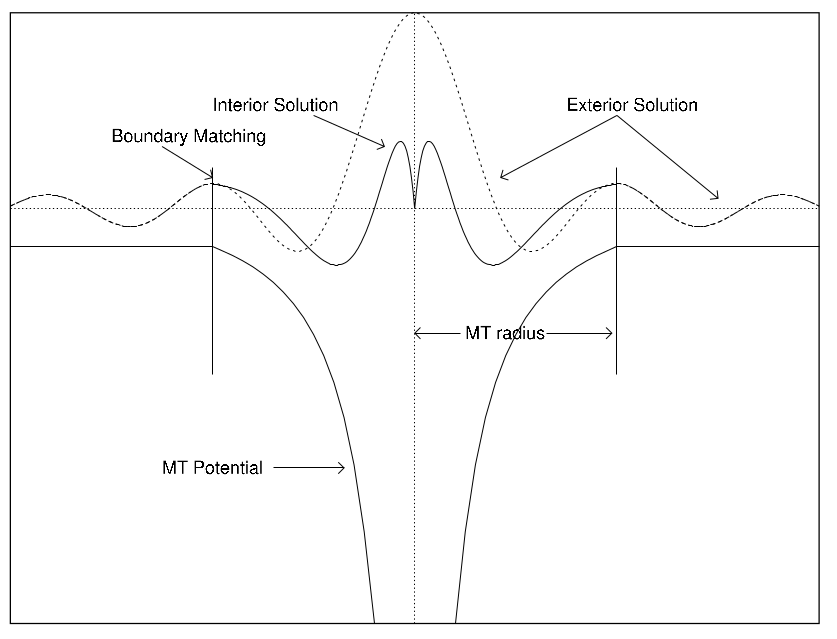
\includegraphics[height=1.25in,width=1.95in,viewport=0 0 845 635,clip]{Figures/MTO-envelope-1.png}
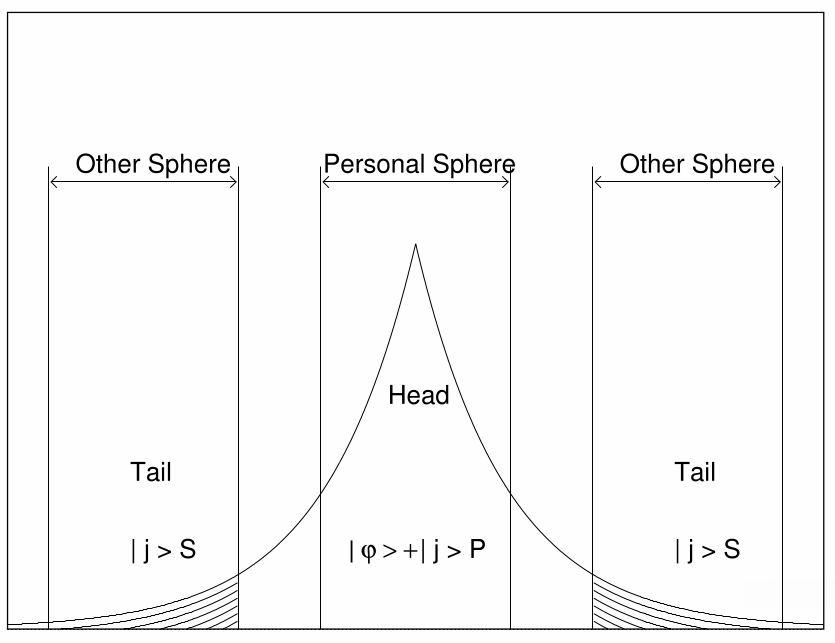
\includegraphics[height=1.25in,width=1.95in,viewport=0 0 885 635,clip]{Figures/MTO-envelope-2.png}
\caption{\tiny \textrm{The radial function of MTO expressed in different region.}}%(与文献\cite{EPJB33-47_2003}图1对比)
\label{MTO-envelope}
\end{figure}
当$q_0=0$时,构成最简单的\textrm{MTO}基函数
		\begin{displaymath}
			\hspace*{-12pt}\chi_L^{\mathrm{MTO}}(\varepsilon,0,\vec r)=\mathrm{i}^lY_L(\hat{\vec r})u_l(\varepsilon,S)\left\{
			\begin{aligned}
				&\dfrac{u_l(\varepsilon,r)}{u_l(\varepsilon,S)}-\dfrac{D_l(\varepsilon)+l+1}{2l+l}\left(\dfrac rS\right)^l&\, r\leqslant S\\
				&+\dfrac{l-D_l(\varepsilon)}{2l+1}\left(\dfrac Sr\right)^{l+1}&\, r>S
			\end{aligned}\right.
		\end{displaymath}
}

\frame
{
	\frametitle{正则能带基函数}
%	\begin{displaymath}
%		\hspace*{-15pt}\begin{aligned}
%			&\left[\dfrac S{|\vec r-\vec R|}\right]^{l+1}\mathrm{i}^lY_L(\widehat{\vec r-\vec R})\\
%				=&4\pi\sum_{L^{\prime}}\bigg[\dfrac rS\bigg]^{l^{\prime}}\mathrm{i}^{l^{\prime}}Y_{L^{\prime}}(\hat{\vec r})\left\{\dfrac{(2l^{\prime\prime}-1)!!}{(2l-1)!!(2l^{\prime}+1)!!}C_{L^{\prime}L^{\prime\prime}}^L\bigg[\dfrac S{|\vec R|}\bigg]^{l^{\prime\prime}+1}\mathrm{i}^{-l^{\prime\prime}}Y_{L^{\prime\prime}}^{\ast}(\hat{\vec R})\right\}
%		\end{aligned}
%	\end{displaymath}

	\textcolor{blue}{考虑平移周期性},
$$\chi_{L,\vec k}^{\mathrm{MTO}}(\varepsilon,0,\vec r)=\sum_{\vec T}\mathrm{e}^{\mathrm{i}\vec k\cdot\vec R}\chi_L^{\mathrm{MTO}}(\varepsilon,0,\vec r)$$
\textcolor{blue}{\textrm{MT}球内的\textrm{MTO-ASA}的基函数为}
{\fontsize{9.0pt}{5.2pt}\selectfont
\begin{displaymath}
	\begin{aligned}
		\chi_{L,\vec k}^{\mathrm{MTO}}(\varepsilon,0,\vec r)=&\underline{\textcolor{red}{u_l(\varepsilon,r)\mathrm{i}^lY_L(\hat{\vec r})}}-\dfrac{D_l(\varepsilon)+l+1}{2l+l}u_l(\varepsilon,S)\left(\dfrac rS\right)^l\mathrm{i}^lY_L(\hat{\vec r})\\
		&+\dfrac{l-D_l(\varepsilon)}{2l+1}u_l(\varepsilon,S)\sum_{L^{\prime}}\left(\dfrac rS\right)^{l^{\prime}}\dfrac1{2(2l^{\prime}+1)}\mathrm{i}^{l^{\prime}}Y_{L^{\prime}}(\hat{\vec r})S_{LL^{\prime}}(\vec k)
	\end{aligned}
\end{displaymath}}
其中
\begin{displaymath}
	\begin{aligned}
		S_{LL^{\prime}}(\vec k)=&2(2l+1)\dfrac{[D_l(\varepsilon)+l+1]}{[D_l(\varepsilon)-l]}\\
		=&C_{l^{\prime}m^{\prime},lm}\sum_{\vec T}\mathrm{e}^{\mathrm{i}\vec k\cdot\vec T}\bigg[\dfrac S{|\vec T|}\bigg]^{l^{\prime\prime}+1}\big[\sqrt{4\pi}\mathrm{i}^{l^{\prime\prime}}Y_{L^{\prime\prime}}(\hat{\vec T})\big]^{\ast}
	\end{aligned}
\end{displaymath}
}

\frame
{
	\frametitle{正则能带}
	\textcolor{red}{$u_l(\varepsilon,r)\mathrm{i}^lY_L(\hat{\vec r})$是\textrm{MT}球内满足原子分波函数的形式}
	\begin{itemize}
		\item \textcolor{blue}{在\textrm{MT}球内来自其他原子尾部贡献部分}$$\dfrac{l-D_l(\varepsilon)}{2l+1}u_l(\varepsilon,S)\sum_{L^{\prime}}\left(\dfrac rS\right)^{l^{\prime}}\dfrac1{2(2l^{\prime}+1)}\mathrm{i}^{l^{\prime}}Y_{L^{\prime}}(\hat{\vec r})S_{LL^{\prime}}(\vec k)$$
		\item \textcolor{blue}{在\textrm{MT}球内非物理贡献部分}$$\dfrac{D_l(\varepsilon)+l+1}{2l+l}u_l(\varepsilon,S)\left(\dfrac rS\right)^l\mathrm{i}^lY_L(\hat{\vec r})$$
	\end{itemize}
	\textcolor{red}{这两部分相互抵消},由此得到\textrm{MTO}中的\textrm{KKR}-型方程
	\begin{displaymath}
		\det[S_{LL^{\prime}}(\vec k)-P_l(\varepsilon)\delta_{LL^{\prime}}]=0
	\end{displaymath}
	这里$P_l(\varepsilon)$是“势函数”
	\begin{displaymath}
		P_l(\varepsilon)=2(2l+1)\dfrac{D_l(\varepsilon)+l+1}{D_l(\varepsilon)-l}
	\end{displaymath}
	\textcolor{blue}{作变换$S_{LL^{\prime}}(\vec k)\xrightarrow{\bf{T}\rm{_u}}S_{lm,lm^{\prime}}(\vec k)$,由此确定的$\varepsilon_l(\vec k)$即正则能带}
}

\frame
{
	\frametitle{\textrm{MTO}轨道的“尾部抵消”}
\begin{figure}[h!]
	\vspace*{-0.7in}
\centering
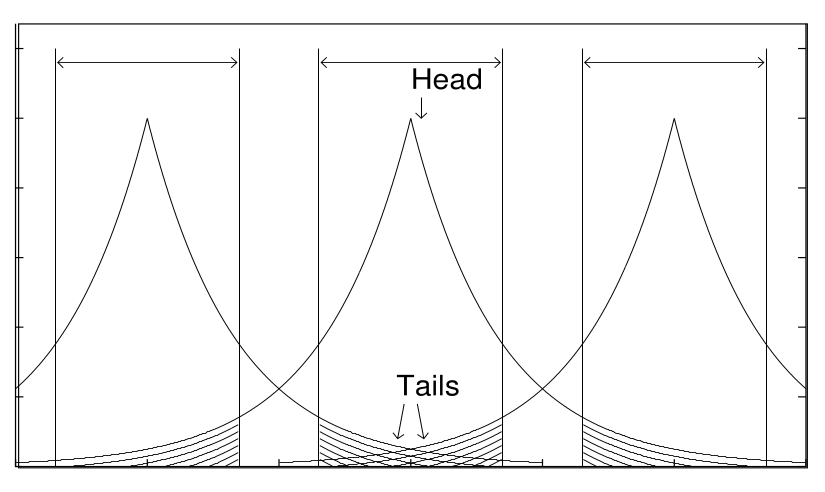
\includegraphics[height=2.55in,width=3.15in,viewport=0 0 845 635,clip]{Figures/MTO-Tail_cancellation.png}
\caption{\tiny \textrm{The wavefunction in the spere at the origin is the sum of the ``head function'' in that sphere plus the tails from neighboring spheres. The schematic illustration of the ``tail cancellation'' of the MTO.}}%(与文献\cite{EPJB33-47_2003}图1对比)
\label{MTO-tail-candellation}
\end{figure}
}

\frame
{
	\frametitle{\textrm{LMTO~.vs.~LAPW}}
\begin{figure}[h!]
\centering
\vspace*{-0.15in}
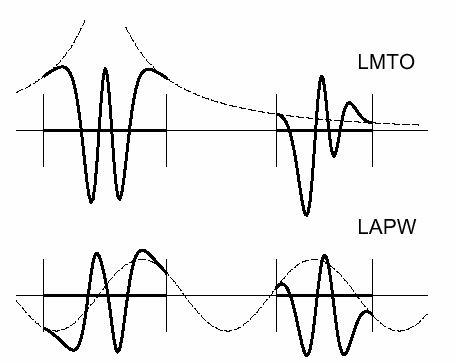
\includegraphics[height=2.50in,width=3.30in,viewport=0 0 440 350,clip]{Figures/LMTO-vs-LAPW.png}
\caption{\fontsize{5.5pt}{4.2pt}\selectfont{\textrm{Schematic illustration of LMTO vs LAPW.}}}%(与文献\cite{EPJB33-47_2003}图1对比)
\label{LMTO-vs-LAPW}
\end{figure}
}

\frame
{
	\frametitle{\textrm{LMTO}方法}
	与\textrm{LAPW}方法类似,在给定能量$\varepsilon_v$和衰减常数$q_0$附近,\textrm{LMTO}的基函数球内部分用函数$\psi_l(\varepsilon_v,r)$及其对能量导数$\dot\psi(\varepsilon_v,r)$表示\\
\textcolor{blue}{\textrm{LMTO}与\textrm{MTO}基函数的区别}
	\begin{itemize}
		\item 球内部分的$\psi(\varepsilon,r)$是主要部分:~由$\psi(\varepsilon_v,r)$和$\dot\psi(\varepsilon_v,r)$线性组合
		\item 球内来自其它\textrm{MT}球的函数尾部贡献被$\dot\psi(\varepsilon_v,r)$的线性组合替代
	\end{itemize}
	由此根据物理直觉,可以把\textrm{LMTO}基函数的形式表示成
		\begin{displaymath}
			\hspace*{-12pt}\chi_L^{\mathrm{LMTO}}(\varepsilon,q_0,\vec r)=\mathrm{i}^lY_L(\hat{\vec r})\left\{
			\begin{aligned}
				&u_l(\varepsilon,r)-q_0\cot(\eta_l(\varepsilon))J_l(q_0r)&\, r\leqslant S\\
				&q_0N_l(q_0r)&\, r>S
			\end{aligned}\right.
		\end{displaymath}
		实际应用中,选定函数$J_l$和$N_l$与球\textrm{Bessel}函数$j_l$和\textrm{Neumann}函数$n_l$相似
}

\frame
{
	\frametitle{\textrm{LMTO}方法}
	根据物理边界要求,在\textrm{MT}球内,基函数$\chi_L^{\mathrm{LMTO}}$对能量$\varepsilon$的导数在$\varepsilon=\varepsilon_v$为0可确定$J_l$
		\begin{displaymath}
			J_l(q_0r)=-\dfrac{\dot{\psi}_l(\varepsilon_v,r)}{q_0\frac{\mathrm{d}}{\mathrm{d}\varepsilon}\cot(\eta_l(\varepsilon_v))},\,r\leqslant S
		\end{displaymath}
		$N_L$的定义与\textrm{Neumann}函数相似,在极限条件$n_l\rightarrow N_l$,$j_l\rightarrow J_l$,其它\textrm{MT}球的函数尾巴满足多重散射展开方式
		\begin{displaymath}
				N_L(q_0,\vec r-\vec R)=4\pi\sum_{L^{\prime},L^{\prime\prime}}C_{L^{\prime}L^{\prime\prime}}^Ln_{L^{\prime\prime}}^{\ast}(q_0,\vec R-\vec R\,^{\prime})J_{L^{\prime}}(q_0,\vec r-\vec R\,^{\prime}),\,r>S
		\end{displaymath}
		由此得到的能量无关的\textrm{LMTO}基函数满足
		\begin{itemize}
			\item \textcolor{blue}{在\textrm{MT}球内函数由$\psi_l$和$\dot{\psi}_l$的线性组合}
			\item \textcolor{blue}{\textrm{MT}球内函数光滑延伸到\textrm{MT}外,并能与其余\textrm{MT}球函数能量导数$\dot{\psi}_l$光滑连续}
		\end{itemize}
}

\frame
{
	\frametitle{\textrm{LMTO}方法}
	对于周期体系,取$q_0=0$~,\textrm{LMTO}方法的基函数可以表示为
	\begin{displaymath}
		\chi_{L,\vec k}^{\mathrm{LMTO}}(\vec r)=\dfrac{\psi_{l-}(\vec r)}{\psi_{l-}(S)}-\dfrac1{\psi_{l+}(S)}\sum_{L^{\prime}}\psi_{l^{\prime}+}(\vec r)\dfrac1{2(2l^{\prime}+1)}S_{LL^{\prime}}(\vec k)
	\end{displaymath}
	这里$\psi_{l-}(r)\equiv\psi_l(D=-l-1,r)$,$(r/S)^l\rightarrow\psi_{l+}(r)\equiv\psi_l(D=l,\varepsilon)$
	$$\psi(D,r)=\psi(r)+\omega(D)\dot\psi(r)$$
	这里
	$$\omega(D)=-\dfrac{\psi(S)D-D(\psi)}{\dot\psi(S)D-D(\dot\psi)}$$
	这里$D(\psi)$和$D(\dot\psi)$分别是$\psi$和$\dot\psi$在\textrm{MT}球面上的对数导数

	由此定义的\textrm{LMTO}基函数
	\begin{itemize}
		\item \textcolor{red}{对能量$\varepsilon_v$依赖到一阶}
		\item \textcolor{red}{径向函数在\textrm{MT}球外的尾巴抵消保持到计算所需要的最低阶}
	\end{itemize}
}

\frame
{
	\frametitle{固体计算方法总结}
\begin{figure}[h!]
\centering
\vspace*{-0.25in}
%\hspace*{-0.80in}
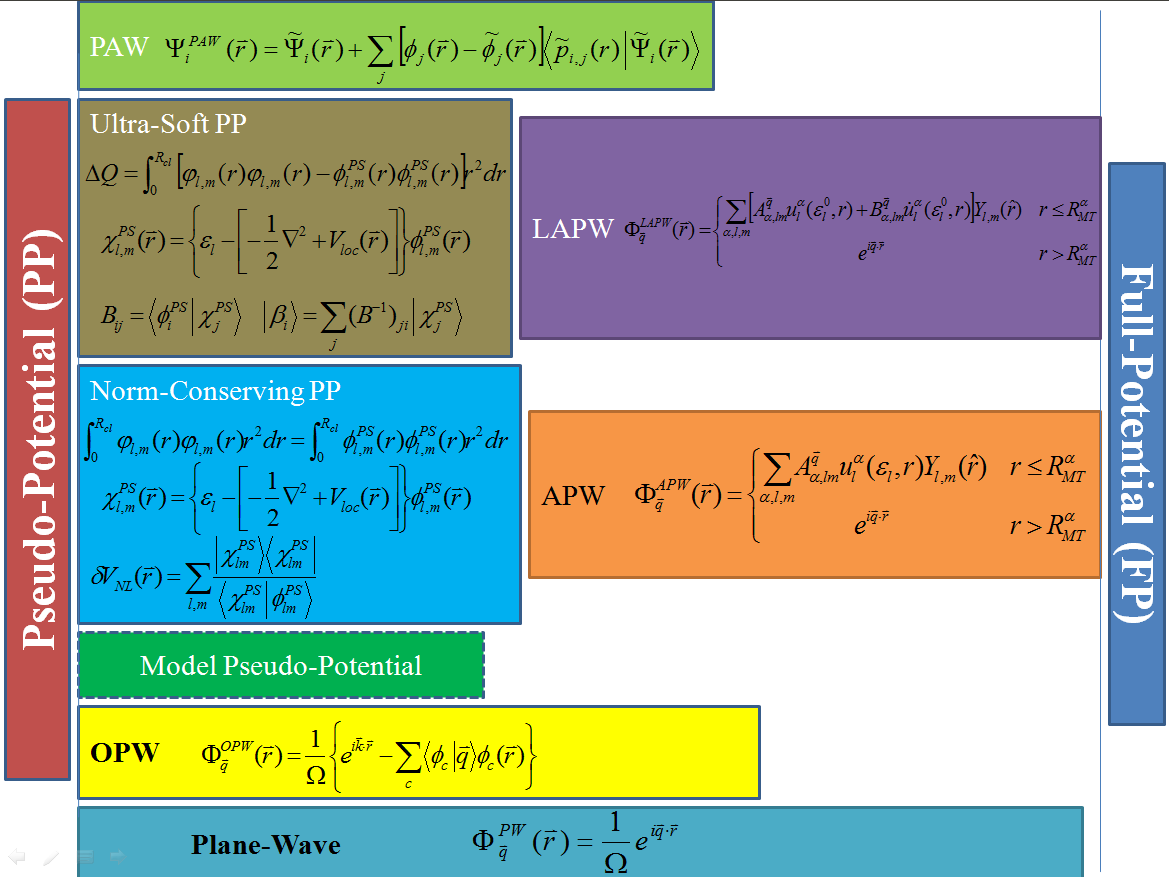
\includegraphics[height=2.80in,width=4.10in,viewport=0 0 1190 876,clip]{Figures/Pseudo-Full_Potential.png}
%\caption{\tiny \textrm{Pseudopotential for metallic sodium, based on the empty core model and screened by the Thomas-Fermi dielectric function.}}%(与文献\cite{EPJB33-47_2003}图1对比)
\label{Pseudo-Full_Poential}
\end{figure}
}

\frame
{
	\frametitle{固体计算软件概览}
\begin{figure}[h!]
\centering
\vspace*{-0.05in}
%\hspace*{-0.80in}
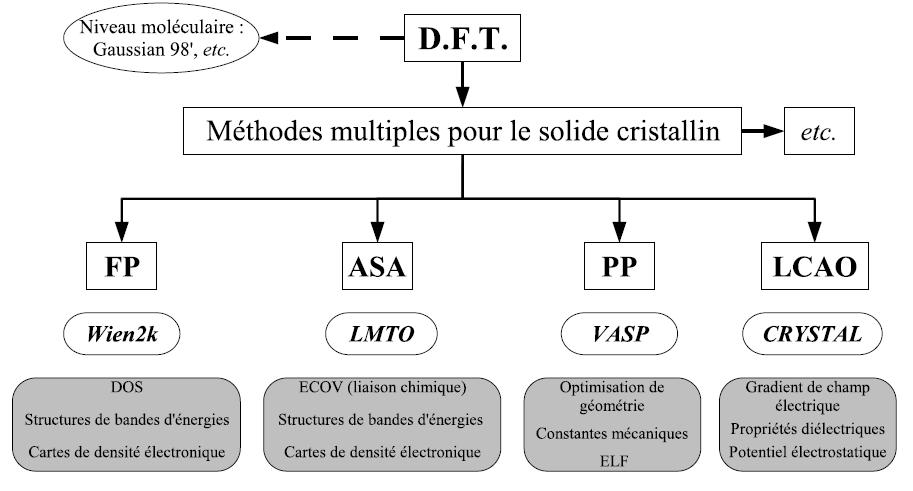
\includegraphics[height=2.30in,width=4.00in,viewport=0 0 920 500,clip]{Figures/DFT-Software.jpg}
%\caption{\tiny \textrm{Pseudopotential for metallic sodium, based on the empty core model and screened by the Thomas-Fermi dielectric function.}}%(与文献\cite{EPJB33-47_2003}图1对比)
\label{Abinitio-Softwares}
\end{figure}
}
%------------------------------------------------------------------------Reference----------------------------------------------------------------------------------------------
		\frame[allowframebreaks]
{
\begin{thebibliography}{99}
\frametitle{主要参考文献}
{\tiny
	\bibitem{Andersen_Book}\textrm{O. K. Andersen. \textit{Computational Methods in Band Theory} (Plenum, New York, USA, 1971)}
	\bibitem{PR43-804_1933}\textrm{E. Wigner and F. Seitz \textit{Phys. Rev.}, \textbf{43} (1933), 804}
	\bibitem{Condon-Shortley}\textrm{E. U. Condon and G. H. Shortley. \textit{The Theory of Atomic Spectra} (University Press, Cambridge, 1951)}
	\bibitem{PR94-1111_1954}\textrm{W. Kohn and N. Rostocker. \textit{Phys. Rev.} \textbf{94} (1954), 1111}
	\bibitem{PRB12-3060_1975}\textrm{O. K. Andersen. \textit{Phys. Rev.} B, \textbf{12} (1975), 3060}
	\bibitem{LMTO_Book}\textrm{H. Skriver. \textit{The LMTO method} (Springer, New York, USA, 1984)}
	\bibitem{Singh}\textrm{D. J. Singh. \textit{Plane Wave, PseudoPotential and the LAPW method} (Kluwer Academic, Boston,USA, 1994)}
	\bibitem{Nemoshkalenko-Antonov}\textrm{V. V. Nemoshkalenko and V. N. Antonov. \textit{Computational Methods in Solid State Physics} (Gordon and Breach Science Publisher, Amsterdam, The Netherlands, 1998)}
}
\end{thebibliography}
\nocite*{}
}
%-----------------------------------------------------------------------------------------------------------------------------------------------------------------------%
